
Webový server je rozdělený do dvou na sobě nezávislých komponent \texttt{user\_interface} a
\texttt{stm\_communication} tak, jak je to znázorněno na obrázku \ref{server-overview}.
\texttt{user\_interface} zprostředkovává veškerou komunikaci mezi uživatelem (klientem) a jeho STM
zařízeními sestávající z nastavování intevalů a čtení aktuálně naměřené teploty.
\texttt{stm\_communication} přijímá aktuálně naměřenou teplotu od STM zařízení a vyměňuje si s nimi intervaly.
Obě komponenty čtou a zapisují data do společné databáze.
Tím je nepřímo zajištěna komunikace mezi uživatelem a jeho zařízením skrz server.

% server-overview obrazek
\begin{figure}[tbh]\centering
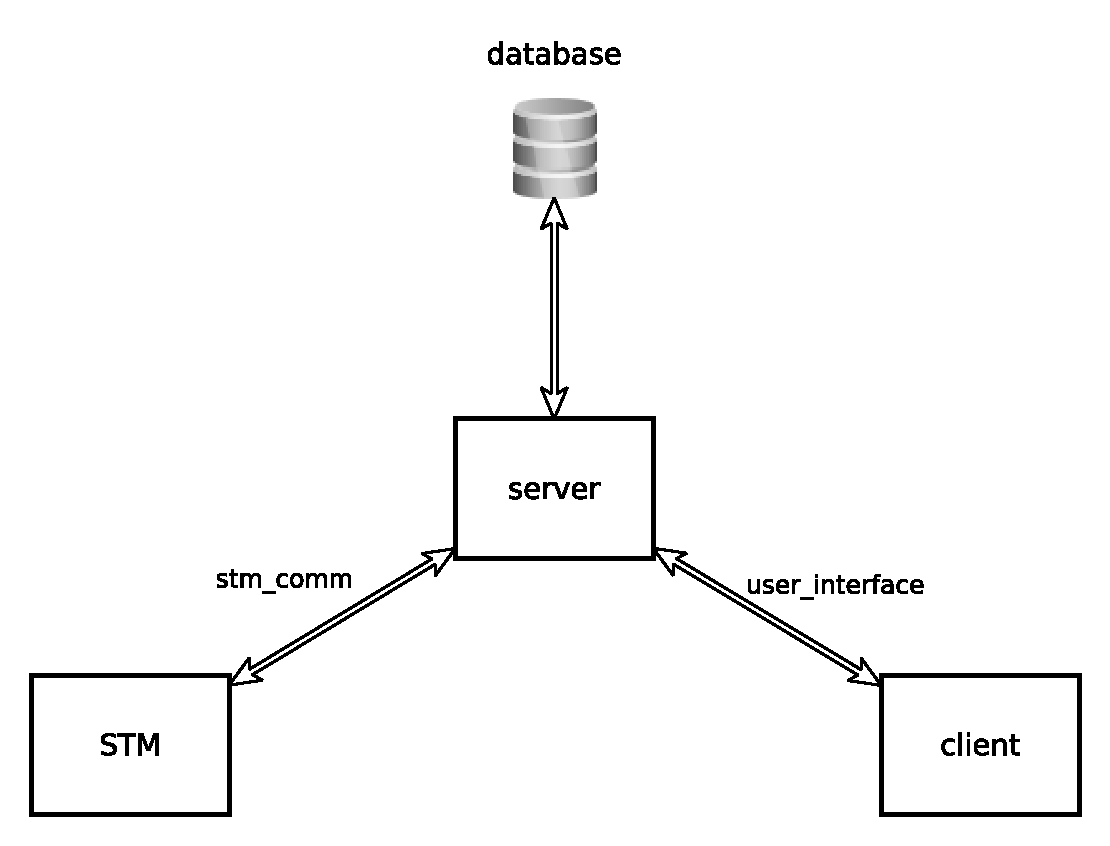
\includegraphics[scale=0.6]{../img/server_overview.pdf}
\caption{Komponenty webového serveru}
\label{server-overview}
\end{figure}

% Použití frontend frameworku by bylo vhodné.
V kapitole analýza jsme se rozhodli použít Django jako backend framework, k vývoji frontend
používáme pouze Bootstrap a jQuery.
Vzhledem k požadované interaktivitě frontend jsme si tímto rozhodnutím trochu zkomplikovali práci.
Kdybychom chtěli přidat další funkcionalitu, jako je například zobrazení historie pro STM,
bylo by vhodné do serveru integrovat nějaký frontend framework.

Samotná implementace frontendu není pro tuto práci příliš důležitá, proto se jí nebudeme zabývat.
Implementace backend už důležitá je, ovšem v porovnání s implementací STM, kde na serveru máme
k dispozici velikou abstrakci, máme zjednodušenou práci.

% Databázové schéma
\subsection{Databázové schéma}

\begin{figure}[tbh]\centering
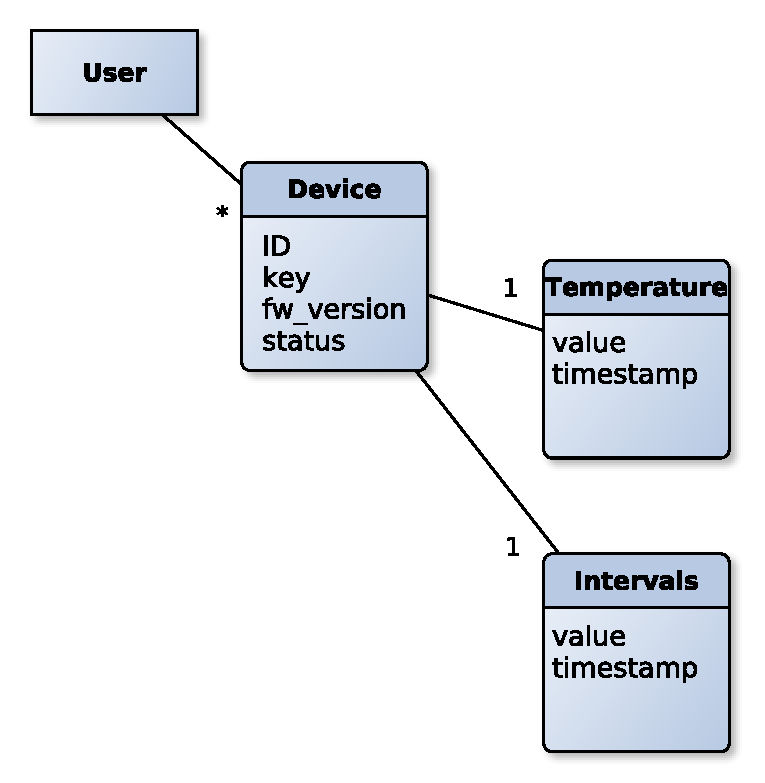
\includegraphics[scale=0.6]{../diagrams/databazove_schema.pdf}
\caption{Databázové schéma}
\label{databazoveschema}
\end{figure}

Databázové schéma \ref{databazoveschema} ukazuje základní objekty a vztahy mezi nimi.

Na server se může registrovat libovolný uživatel zadáním uživatelského jména, hesla a potvrzením
emailové adresy.
Každý uživatel si může přidat omezeně mnoho zařízení.
Každé STM zařízení má svoje ID přiřazeno ještě před tím, než se dostane uživateli do ruky.
Kromě toho, že toto ID je uloženo v databázi na serveru, je potřeba aby bylo zakódovano do firmware
konkrétního STM, což by neměl být problém.
Každé STM má také přiřazenou verzi firmware, to z důvodu že by STM mohlo být teoreticky aktualizováno
na dálku - viz \cite{FW-update-over-ethernet}.
Server a ani STM toto ale zatím nepodporují.
\texttt{status} může být buď \texttt{connected} nebo \texttt{offline}.
\texttt{key} se k STM přiřadí až po tom, co se poprvé přihlásí k serveru.

Co se týká jednotlivých položek, v našem případě \texttt{Temperature} a \texttt{Intervals}, tak ty se
dělí na dva typy - \emph{actual} a \emph{config}.
Actual položky jsou takové, které STM periodicky posílá na server a ten má za úkol je zobrazit uživateli.
Config položky nejsou pouze ke čtení, ale i k zápisu.
Config položky jsou synchronizovány mezi serverem a STM tak, že na obou stranách platí pouze hodnota s
novějším timestampem.
Každá položka v databázi má svůj timestamp a \texttt{value}.
Temperature představuje teplotu, tedy jeho value je prostě číslo.
Na druhou stranu Intervals představuje nastavení teplot po různé časové intervaly, což znamená, že ve
value musí být uložená nějaká komplikovanější hodnota než je číslo.
Vhodné řešení je ukládat do intervals textový řetězec v JSON formátu, zejména kvůli tomu, že v rámci
Pythonu a Javascript se JSON řetězec velice jednoduše parsuje.


